% Teilauswertung X

\newpage
\section{Absorption und Dispersion einer Jodlinie}


\begin{figure}[h]
    \centering
    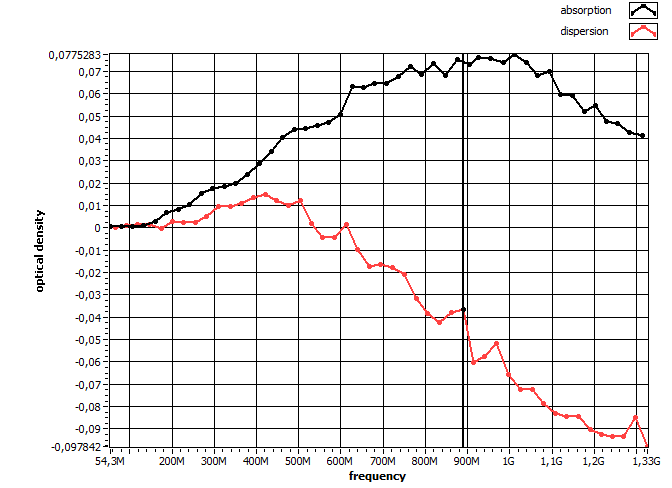
\includegraphics[width=0.75\textwidth]{Bilder/Jodlinie/Gruppe32020Iododgraph1 Kopie.png}
    \caption[Iodlinie]{Iodlinie (Ersatzmessung, Gruppe 3, 2020)}
    \label{fig:IodlinieG32020}
\end{figure}

%\subsection{Nachprüfen der Absorption}

Zur Nachprüfung des berechneten Absorptionssignals wurden bei drei Frequenzen manuell eine Messung mit und ohne Probe durchgeführt. Die optische Dichte wurde mit folgender Formel berechnet.
\begin{align}
    OD = \frac{\Delta U}{U_\mathrm{A}} \cdot OD_\mathrm{FPI}
\end{align}
Wobei $\Delta U$ die Spannungsdifferenz der Basislinien der Messungen mit und ohne Zelle ist, $U_\mathrm{A}$ die Höhe der einfachen Peaks der Messungen mit der Zelle und $OD_\mathrm{FPI} = 0,09 \pm 0,07$ die optische Dichte des FPI.
\begin{table}[h]
    \centering
    \begin{tabular}{c|cc|c}
        $\omega_m$/MHz & $\Delta U$ / mV & $\Delta U_\mathrm{A}$ / mV & OD \\ \hline
        79,7 & $3 \pm 4$ & $131 \pm 4$ & $0,002 \pm 0,003$  \\
        491,9 & $150 \pm 4$ & $269 \pm 4$ & $0,05 \pm 0,04$ \\
        989,1 & $320 \pm 4$ & $283 \pm 4$ & $0,10 \pm 0,08$ \\
    \end{tabular}
    \caption{Ergebnisse für manuelle Messung der optischen Dichte.}
    \label{tab:ODIod}
\end{table}

Betrachtet man die Werte aus der Tabelle \ref{tab:ODIod}, für die optische Dichte, so fällt auf, dass diese im Rahmen des Fehlers mit dem in Abbildung \ref{fig:IodlinieG32020} gezeigten werten übereinstimmen. 

Hier wurde mit einem Korrekturfaktor von 2,22 gearbeitet, da unsere Rechteckfunktion aber eher Trapezförmig ist und die Ecken etwas abgerundet sind, weicht der Wert des Faktors wohl etwas nach unten ab.

Für die Vakuumwellenlänge der Iodlinie gilt:
\begin{gather}
    \lambda = \frac{c_0}{f} = (632,9915 \pm 0,0004) \, \text{nm}
\end{gather}
In Luft ($n_{Luft} = 1,0003$) gilt:
\begin{gather}
    \lambda_{Luft} = \frac{\lambda}{n_{Luft}} = (632,8017 \pm 0,0004)\, \text{nm}
\end{gather}

Aus dem Diagramm konnte Breite der Jodlinie, am halben Maximalwert, von ca. 848MHz abgelesen werden.
Für die Dopplerbreite gilt:
\begin{gather}
    \delta f = \frac{f_0}{c} \sqrt{\frac{8 k_B T ln2}{m}}
\end{gather}
In unserem Fall git: $f_0 \approx 880$ MHz,  $T \approx 294$ K und $m = 2 \cdot 126,9 u$.
\begin{gather}
    \Rightarrow \delta f \approx 678 \, \text{MHz}
\end{gather}
Es fällt auf, dass der ermittelte Wert merklich größer ist als der theoretische. Dies liegt daran, dass es eine nicht aufgelöste Hyperfeinstruktur gibt, deren Komponenten ebenfalls eine Dopplerverbreiterung erfahren.


Im folgenden soll aus den Extremwerten der Phasenänderung $\Delta \Phi$ die Brechungsindexänderung $\Delta \eta$ berechnet werden. Folgende Formel wird dafür genutzt:
\begin{gather}
    \Delta \eta = \Delta \Phi \frac{\lambda}{2 \pi L}
\end{gather}
Es gilt: $\Delta \Phi \approx 0,11$. Daraus folgt:
\begin{gather}
    \Delta \eta \approx 2,8 \cdot 10^{-8}
\end{gather}

Betrachtet man den Nulldurchgang des Dispersionssignales so fällt auf, dass er vor dem Peak des Absorptionssignales liegt. Bei gültigen Kramer-Kronig-Relationen würde man erwarten das sich diese Punkte übereinander befinden. Dies kann möglicherweise durch eine Leistungsverbreiterung der Linien verursacht worden sein. Diese würde dazu führen, dass die mathematischen Voraussetzungen für die Gültigkeit der Relationen nicht erfüllt wären.
Außerdem ist der Verlauf der Absorptionslinie bezüglich des Nulldurchgangs auffallend, bei gültigen Kramers-Kronig-Relationen würde man einen symmetrischen Verlauf erwarten.
